\begin{myblock}{MS-lite: A Lightweight M\&S}
\Large
\begin{itemize}
\item MS-lite is extremely fast in construction by design:
\end{itemize}

\hspace*{0.5in}
\begin{minipage}{\textwidth}
\begin{itemize}
\item random merge order
\item minimal \embl{$h$-preserving} shrinking
\item no label reduction
\end{itemize}
\end{minipage}

\begin{center}
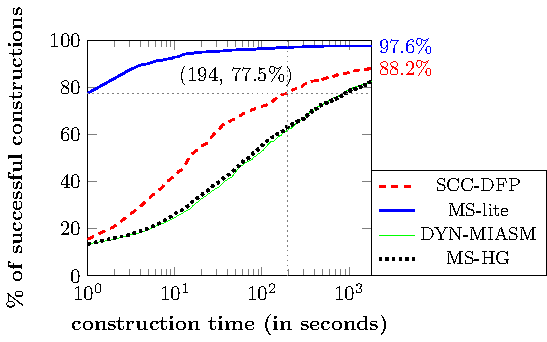
\includegraphics[scale=2.5]{pdfs/time-cdf-figure0.pdf}
\end{center}
%\begin{minipage}{\textwidth}
%  \centering
%  \raisebox{-0.5\height}{}
%\end{minipage}

\begin{itemize}
\item \embl{Complementary strength} of MS-lite:
\end{itemize}

\begin{minipage}{\textwidth}
  \centering
  \raisebox{-0.5\height}{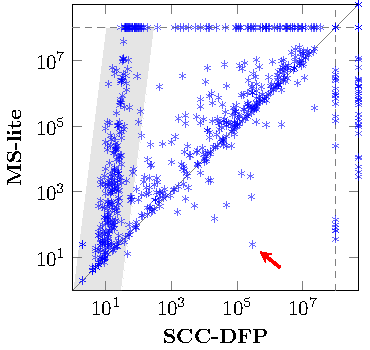
\includegraphics[scale=2.3]{pdfs/figure2.pdf}}
  \hspace*{0.5in}
  \raisebox{-0.5\height}{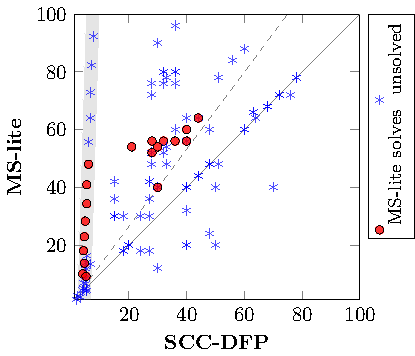
\includegraphics[scale=2.3]{pdfs/figure3.pdf}}
\end{minipage}

\end{myblock}


\begin{myblock}{Combining MS-lite and MS-HG}
\Large
\begin{itemize}
\item Taking maximum of two heuristics, i.e., $h(s)=\max(h_1(s), h_2(s))$, during search.
\item Build MS-lite and another "normal" M\&S, but terminate the construction if it takes too much memory/time.
\end{itemize}


\begin{minipage}{0.45\textwidth}
\begin{itemize}
\item Results:
\end{itemize}
\end{minipage}
\begin{minipage}{0.45\textwidth}
\begin{itemize}
\item Taxonomy:
\end{itemize}
\end{minipage}

\vspace*{0.5in}
\begin{minipage}{0.45\textwidth}
\begin{table}[]
\normalsize
\begin{tabular}{|c|c|c|c|} 
\hline\Tstrut 
 SD & MS-HG & Lite-SD & Lite-HG \\
 \hline\Tstrut 
 \ 671\  & +10 & +47.8 & +75.2 \\
  \hline
 % 718.8$\pm0.5$ & 746.2$\pm0.8$
\end{tabular}
\end{table}
\hspace*{-0.4in}
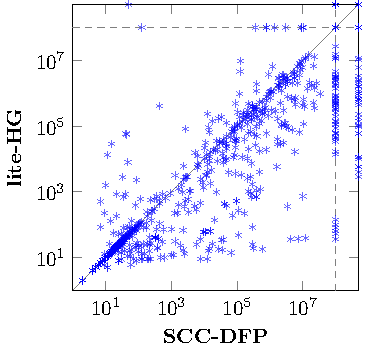
\includegraphics[scale=2.5]{pdfs/figure6.pdf}
\end{minipage}
\begin{minipage}{0.5\textwidth}
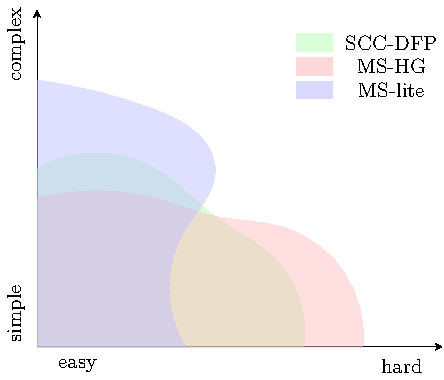
\includegraphics[scale=2.5]{pdfs/taxonomy.pdf}
\normalsize
\begin{itemize}
\item $x$-axis: how hard for state space search?
\item $y$-axis: how complex for creating (M\&S) heuristic?
\end{itemize}
\end{minipage}


\end{myblock}

%\begin{myblock}{Taxonomy}
%\Large
%\begin{itemize}
%\item draw taxonomy \placeholder{1000pt}{600pt}
%\end{itemize}
%
%\end{myblock}


